\paragraph{arithmetic\_u32}

U32ArithmeticGate gate is used for compute $\text{res} = \text{mul\_0} \times \text{mul\_1} + \text{add}$. Res is store in res\_lo and res\_hi each of which can be represented by 15 limbs.

Gate structure is like \figref{fig:arithmetic-u32}.

\begin{figure}[!ht]
    \centering
    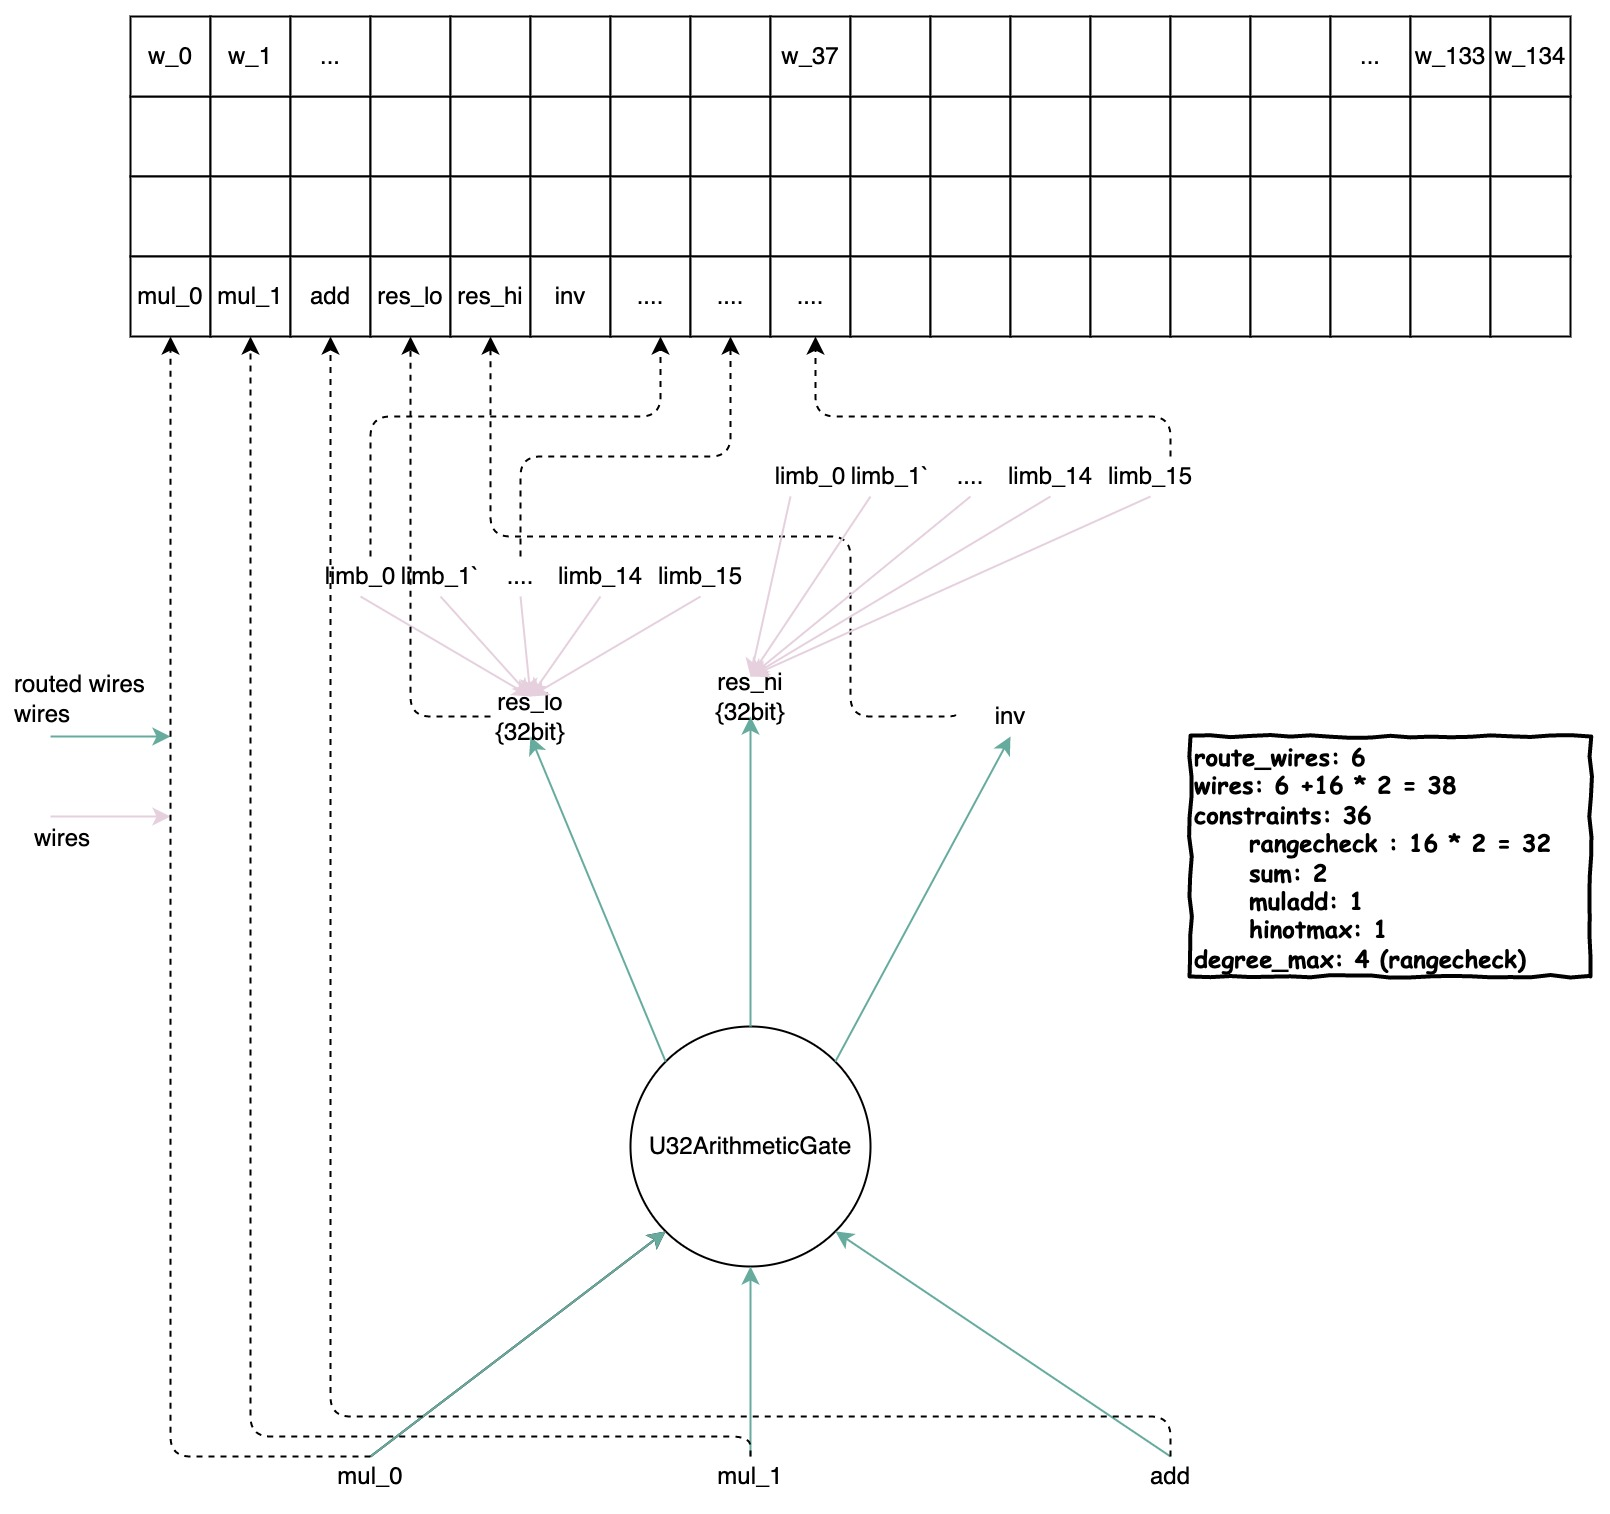
\includegraphics[width=0.8\textwidth]{gates/arithmetic_u32.jpeg}
    \caption{U32ArithmeticGate}
    \label{fig:arithmetic-u32}
\end{figure}

Constraints for each operation:
\begin{itemize}
    \item Constrain res is not overflow (less equal than \verb|max_u32 * max_u32 + max_u32|). -- 1 constraint with degree 2.
    \item Constrain combined((by res\_lo and res\_hi)) output equals computed (by \verb|mul_0 * mul_1 + add|) output. -- 1 constraint with degree 2.
    \item Limbs range check. -- 32 (limbs) constraints with degree 4. (limbs are all 2-bits)
    \item Constrain limbs for res\_lo and res\_hi. -- 2 constraints with degree 1.
\end{itemize}

In summary, there are 36 constraints for each operation. Degree of the gate is 4 which is needed by 4-bits limbs range check.
